
%----------------------------------------------------------------------------------------
%	Lecture 24
%----------------------------------------------------------------------------------------

\chapter{Normal Vector to a Surface} 

\bigbreak

\section{Normal Vector for a Surface : $z = f(x, y)$}

For a surface $z = f(x, y)$, we have $\hat{n} = \pm \left< -f_x, -f_y, 1 \right> dx dy$.
We need to figure out the normal vector for a small rectangle on the $XY$-plane projected onto our surface.
If the rectangle in the $XY$-plane is small enough then the projected area will be a parallelogram.
And we can find the area of the parallelogram by taking the cross product of its sides.


Let the sides of the parallelogram be ${\bf u}$ and ${\bf v}$.
Such that ${\bf u}$ corresponds to moving $dx$ along $x$-axis.
And ${\bf v}$ corresponds to moving $dy$ along the $y$-axis. 
So our area will be $\hat{n} dS = {\bf u} \times {\bf v}$. 
Now ${\bf u} = \left< dx, 0, dz \right>$ as $y$ is constant along the $x$-axis.
Similarly, ${\bf v} = \left< 0, dy, dz \right>$. 

By linear approximation, we can say that ${\bf u} = \left< dx, 0, f_x dx \right>$
and ${\bf v} = \left< 0, dy, f_y dy \right>$ because $z = f(x, y)$.
We can factor out $dx$ and $dy$ as ${\bf u} = \left<1, 0, f_x \right> dx$ and ${\bf v} = \left< 0, 1, f_y \right> dy$
Now,

\begin{align*}
{\bf u} \times {\bf v} & = (\left< 1, 0, f_x \right> \times \left< 0, 1, f_y \right> ) dx dy \\
& =
\begin{vmatrix*}
    \hat{i} & \hat{j} & \hat{k} \\
    1 & 0 & f_x \\
    0 & 1 & f_y
\end{vmatrix*} dx dy \\
& = (\ijk{-f_x}{-f_y}{1}) dx dy \\
& = \left< -f_x, -f_y, 1 \right> dx dy
\end{align*}

Now we have a plus-minus because its upto us to decide to choose from the two normal vectors.


{\bf Example : } Let's say we want to find the flux ${\bf F} = z \hat{k}$ 
through the potion of the paraboloid $z = x^2 + y^2$ above the unit disk.

Let's say we want the normal vector pointing upwards.
We have $z = f(x, y) = x^2 + y^2$ so $f_x = 2x$ and $f_y = 2y$
From the last section we have, $\hat{n}dS = \left< -f_x, -f_y, 1 \right> dx dy = \left< -2x, -2y, 1 \right> dx dy$.
\begin{align*}
Flux & = \iint_S z \hat{k} \cdot \hat{n} dS \\
    & = \iint_S z \hat{k} \cdot (\ijk{-2x}{-2y}{1}) dx dy \\
    & = \iint_S z dx dy
\end{align*}

Now we are only concerned with points on the surface so we can use $z = x^2 + y^2$.
Thus our integral will be a regular double integration.
$$ \iint_S x^2 + y^2 dx dy $$

Now we can use the polar coordinates. The range of $x$ and $y$ will be over the unit circle as given.

$$ \int_0^{2\pi} \int_0^1 r^2 r dr d\theta = \int_0^{2\pi} \frac{r^4}{4} \Big|_0^1 d\theta = \int_0^{2\pi} \frac{1}{4} d\theta = \frac{\pi}{2} $$

\section{Normal Vector for a Surface given by Parametric Equations}

Let's say you can't express the surface as $z = f(x, y)$.
And you are given parametric equations $x = x(u, v)$, $y = y(u, v)$ and $z = z(u, v)$ or we can take a position vector ${\bf r} = {\bf r}(u, v)$.
We know that since our surface is 2D we can express it in terms of two variables.
Since we are given equations in terms of $u$ and $v$ we want to setup our integral in terms of $du$ and $dv$.
So we want express $\hat{n}dS$ in terms of $du dv$. 

In the last section we changed $x$ and $y$ and uplifted that to the surface to get a parallelogram.
Here we can do the same with $u$ and $v$ dividing the surface into a grid where the grid lines represent that one of $u$ or $v$ is constant along those lines.

So if we change $u$ then we move ${\bf r}_u du = \left< x_u, y_u, z_u \right> du$.
And if we change $v$ the we move ${\bf r}_v dv = \left< x_v, y_v, z_v \right> dv$.
These two vectors corresponds to a parallelogram on the surface as we take smaller and smaller changes.

So our area $\hat{n}dS = \pm ({\bf r}_u \times {\bf r}_v) du dv$.


\section{Normal Vector for a Surface : $f(x, y, z) = 0$ }

Let's say you are given a surface of the form $f(x, y, z) = 0$.
Its normal vector is the gradient vector of $f$ : ${\bf N} = \nabla f$.

\begin{figure}[ht!]
    \centering
    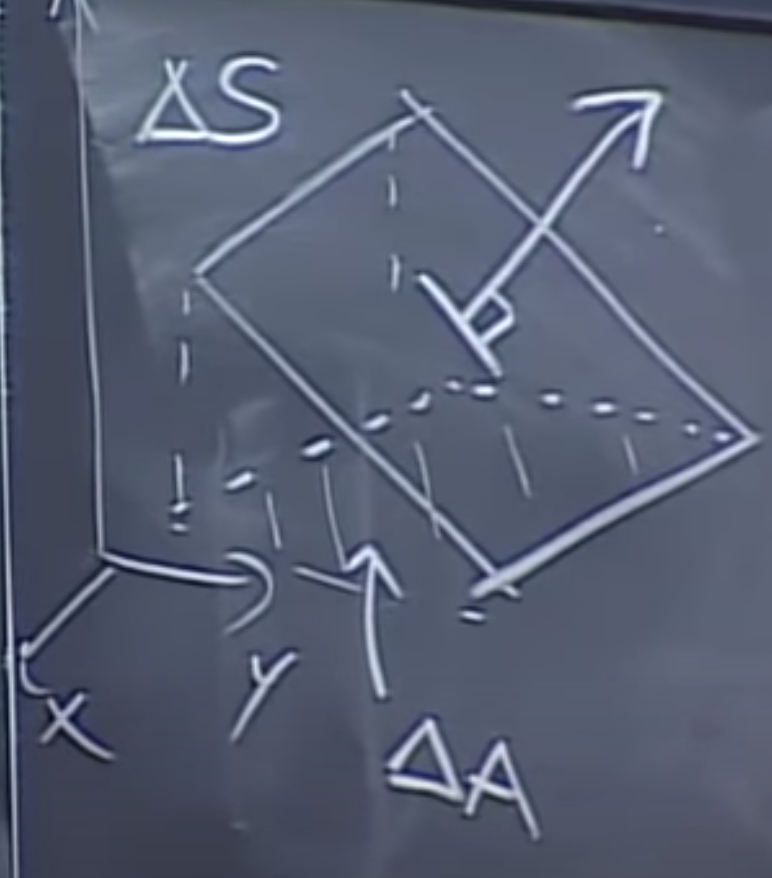
\includegraphics[scale=0.5]{./images/lecture_24_figure_1.png}
    \caption{Projecting Area onto $XY$-plane}
\end{figure}

Now we know that $dA = dx dy$. And we want to find out $dS$ in terms of $dx$ and $dy$.
Let's say that the angle between the slanted plane and the horizontal plane is $\alpha$.
We can see that one of the sides of the rectangle stays the same while the other will get shrinked by a factor of $\cos \alpha$.
Thus, $dA = dS \cos \alpha$.

We can also say that the angle between the normal vectors of $dS$ and $dA$ is also $\alpha$.
So,
$$ 
{\bf N} \cdot \hat{k} = |{\bf N}| |\hat{k}| \cos \alpha 
\Rightarrow \cos \alpha = \frac{ {\bf N} \cdot \hat{k} }{|{\bf N}|}
$$
$$
dS = \frac{dA}{\cos \alpha} = \frac{|{\bf N}|}{{\bf N} \cdot \hat{k}} dx dy 
$$

Note that we don't have to project on the $XY$-plane. We can project onto any plane but we'll have to use the normal vector of that plane instead of $\hat{k}$.

Now, $$ \hat{n} dS = \frac{ |{\bf N}| \hat{n} }{ {\bf N} \cdot \hat{k} } dx dy $$
Now, $|{\bf N}|\hat{n} = \pm {\bf N}$ as $\hat{n}$ is parallel to the normal vector of the surface.
So we get $$\hat{n}dS = \pm \frac{ {\bf N} }{ {\bf N} \cdot \hat{k} } dx dy $$

{\bf Example : } Let the surface be $g(x, y, z) = z - f(x, y) = 0$.

So ${\bf N} = \nabla g = \left< - f_x, - f_y, 1 \right>$
Now, ${\bf N} \cdot \hat{k} = 1$ so $ \hat{n} dS = \pm \left< - f_x, - f_y, 1 \right> dx dy$.

